\documentclass{article}


% if you need to pass options to natbib, use, e.g.:
%     \PassOptionsToPackage{numbers, compress}{natbib}
% before loading neurips_2023


% ready for submission
\usepackage[preprint]{neurips_2023}


% to compile a preprint version, e.g., for submission to arXiv, add add the
% [preprint] option:
%     \usepackage[preprint]{neurips_2023}


% to compile a camera-ready version, add the [final] option, e.g.:
%     \usepackage[final]{neurips_2023}


% to avoid loading the natbib package, add option nonatbib:
%    \usepackage[nonatbib]{neurips_2023}


\usepackage[utf8]{inputenc} % allow utf-8 input
\usepackage[T1]{fontenc}    % use 8-bit T1 fonts
\usepackage{hyperref}       % hyperlinks
\usepackage{url}            % simple URL typesetting
\usepackage{booktabs}       % professional-quality tables
\usepackage{amsfonts}       % blackboard math symbols
\usepackage{nicefrac}       % compact symbols for 1/2, etc.
\usepackage{microtype}      % microtypography
\usepackage{xcolor}         % colors
\usepackage{graphicx}
\usepackage{subcaption}

\title{Theory and Methods for the Ferromagnetic Ising Model}


% The \author macro works with any number of authors. There are two commands
% used to separate the names and addresses of multiple authors: \And and \AND.
%
% Using \And between authors leaves it to LaTeX to determine where to break the
% lines. Using \AND forces a line break at that point. So, if LaTeX puts 3 of 4
% authors names on the first line, and the last on the second line, try using
% \AND instead of \And before the third author name.


\author{
    Jay Shen \\
    Department of Physics \\
    University of Chicago\\
    Chicago, IL 60637 \\
    \texttt{jshe@uchicago.edu} \\
    \And
    Mark Lee \\
    Department of Statistics \\
    University of Chicago\\
    Chicago, IL 60637 \\
    \texttt{markyl@uchicago.edu} \\
}


\begin{document}

\graphicspath{ {../graphics} }

\maketitle

\begin{abstract}

The Ising model is a historically important problem in statistical mechanics. 
Although it was originally proposed as a crude approximation of ferromagnetic 
phenomena, it furnished statistical mechanics, and later probabilistic science 
as whole, with a new paradigm of graph-based modeling that would prove 
influential.
Especially in the distilled, theoretical study of probabilistic graphical 
models (PGMs), which today is its own field, many methods developed for Ising models 
and spin-glasses have been repurposed and reinterpreted, as have the rich 
physical vocabulary of energies, entropy, and partition functions. 

In this paper, we pay homage to the Ising model by applying modern methods to 
the original problem of ferromagnetism. 
We discuss the theory of the Ising model both from a PGMs and statistical 
mechanics point of view, examining the correspondence. 
We then evaluate two approaches to inference—Markov Chain Monte Carlo and
belief propagation. 
Finally, we show the successes and limitations of the Ising model in the context 
of physical phenomena. 

\end{abstract}










\section{Theory of the Ising Model}

The prevailing physical theory explains magnetism as a consequence of the intrinsic 
spin of particles. 
This spin produces a magnetic dipole moment $\vec{\mu}$ proportional to the 
spin $\sigma$:
\[\vec{\mu} = \mu \sigma\]
If an external magnetic field $\vec{B}$ is present, the potential energy is 
given by the classical formula:
\[U_B = - \vec{\mu} \cdot \vec{B}\]
Handily, this also absorbs the splitting of atomic energy levels due to quantum 
mechanical phenomena. 

There also exists a pairwise interaction between particles due to the mutual 
effects of their magnetic moments.
These exchange effects have strength defined by constants $J_{ij}$, 
The potential energy of these pairwise interactions is then:
\[U_{ij} = - J_{ij} \vec{\mu_i} \cdot \vec{\mu_j}\]
Here, we ignore quantum mechanical spin-spin coupling and exclusion energies. 

Note that both potential energies are minimized when the moments align with 
$\vec{B}$ and with each other. 
This corresponds to the theory of ferromagnetism as a systematic alignment of 
spins. 

Now, consider a collection of particles $\vec{\mu_i}$ in the prescence of an 
external magnetic field $\vec{B}$. 
The Hamiltonian, which specifies the total energy of the system, is defined by 
the sum of all pairwise and unary energies:
\begin{equation}\label{exactE}
    E(\vec{\mu}) = -\frac{1}{2}\sum_i \sum_j J_{ij} \vec{\mu_i} \cdot \vec{\mu_j} - \sum_i \vec{\mu_i} \cdot \vec{B}
\end{equation}
In most cases, working with this Hamiltonian is intractable. 
Luckily, we can simplify it by making several strategic assumptions. 

First, in the context of an atomic lattice, all relevant particles are fermionic 
and have spin-$\frac{1}{2}$. 
We assume that all particles within an atom have identical spin, so the spin of 
each atom as a whole is fermionic. 
Then the magnetic moments simplify to $\vec{\mu_i} = \mu \sigma_i$, where 
$\sigma_i \in \{-1, 1\}$ is the atomic spin. 

Second, we make a mean-field nearest-neighbor approximation so that the strength 
of pairwise interactions are negligible for non-adjacent pairs. 
We also assume all non-negligible $J_{ij}$'s are equivalent, that is that the 
material is organized in a regular lattice. 

Coalescing constants, the Hamiltonian reduces nicely to:
\begin{equation}\label{isingE}
    E(\vec{\sigma}) = -J\sum_i \sum_{j \in adj(i)} \sigma_i \sigma_j - \sum_i \sigma_i B_i
\end{equation}
The Boltzmann distribution give a probability of some state $\vec{\sigma}$ at 
inverse temperature $\beta$:
\begin{equation} \label{boltzmann}
    P(\vec{\sigma}) = \frac{1}{Z}e^{-\beta E(\vec{\sigma})} 
\end{equation}
The physical theory of the Ising model has now been developed and we can turn to 
inference as a pure PGMs task. 










\section{Inference on Ising Models}










In many cases, the Ising model of ferromagnetism is used to produce physical 
measurables like energy and magnetization. 
For example, Ernst Ising's original inquiry asked if the Ising model was capable 
of demonstrating phase transitions—changes in the magnetic state due to external 
conditions. 

Now, these measurables require marginal distributions in order to compute, for 
example, the unary and pairwise energies. 
We will now examine two approaches to computing these marginals—Markov Chain 
Monte Carlo and belief propagation. 





\subsection{Markov Chain Monte Carlo}





Monte Carlo algorithms produce better and better estimates by repeated sampling 
from the true distribution. 
When the true distribution is not immediately available for sampling, employing 
Markov Chain Monte Carlo defines an approximate distribution that hopefully, 
during sampling, approaching the true distribution. 

In the context of the Ising model, the Markov states proceeding from some state 
of spins $\vec{\sigma}$ are created by flipping any spin $\sigma_i$ in 
$\vec{\sigma}$. 
We can sample from these states by choosing a random $\sigma_i$ to flip. 
Since we want to move towards the true, equilibrium distribution, we only 
transition to the new state $\vec{\sigma}'$ if 
$P(\vec{\sigma}') > P(\vec{\sigma})$. 
Using the formula for the Boltzmann distribution, this criterion is equivalent 
to $E(\vec{\sigma}') < E(\vec{\sigma})$. 

In practice, we will compute the change in energy 
$\Delta E = E(\vec{\sigma}') - E(\vec{\sigma})$, which has a nice form:
\[
    \Delta E = E(\vec{\sigma}') - E(\vec{\sigma}) = 2 \sigma_i (J \sum_{j \in adj(i)} \sigma_j + B_i)
\]
If $\Delta E < 0$, we transition states. 
If $\Delta E \geq 0$, we will transition states with probability defined by the 
Boltzmann factor:
\[
    \frac{P(\vec{\sigma}')}{P(\vec{\sigma})}
    = e^{-\beta \Delta E} 
\]
This nicely models the phenomena of spin flips caused by field fluctuations. 

We implemented this process in Python on square lattices of spins. 
For our sampling process, we iterated through all spins in random order, at each 
step evaluating the transition defined by flipping the present spin. 
We believe this best simulates the actual equilibration process. 

\begin{figure}
    \begin{subfigure}{\textwidth}
        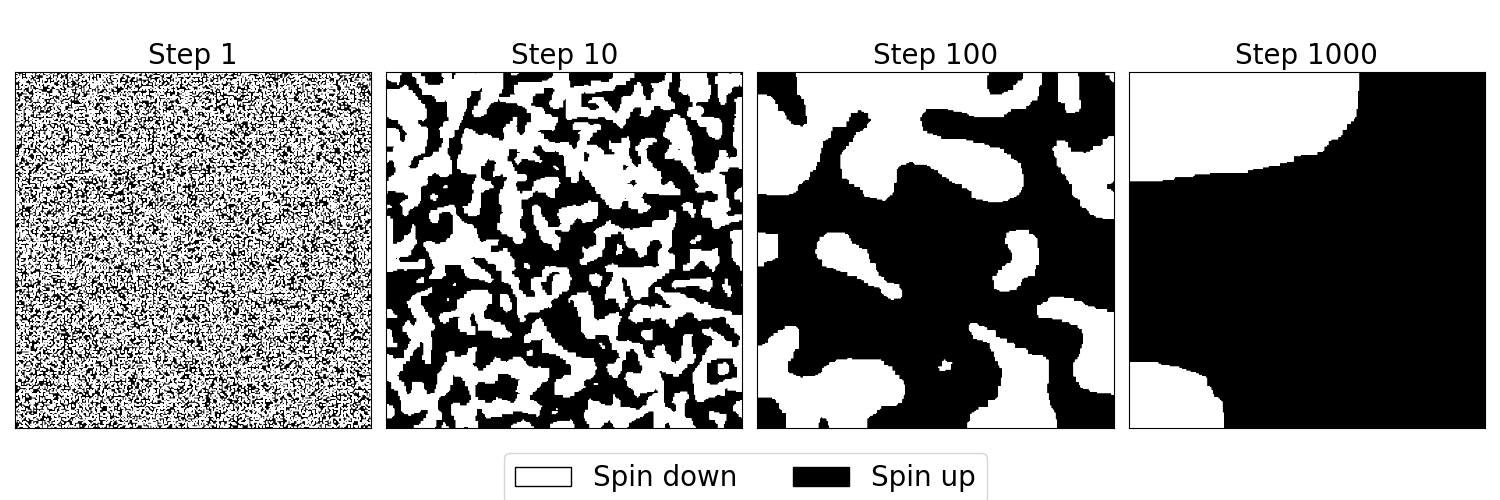
\includegraphics[width=\textwidth]{report_mcmc_gaussian}
        \centering
        \caption{\textit{Spin lattice samples from various points in the sampling process}}
        \label{fig:mcmc_gaussian_a}
    \end{subfigure}
    \begin{subfigure}{\textwidth}
        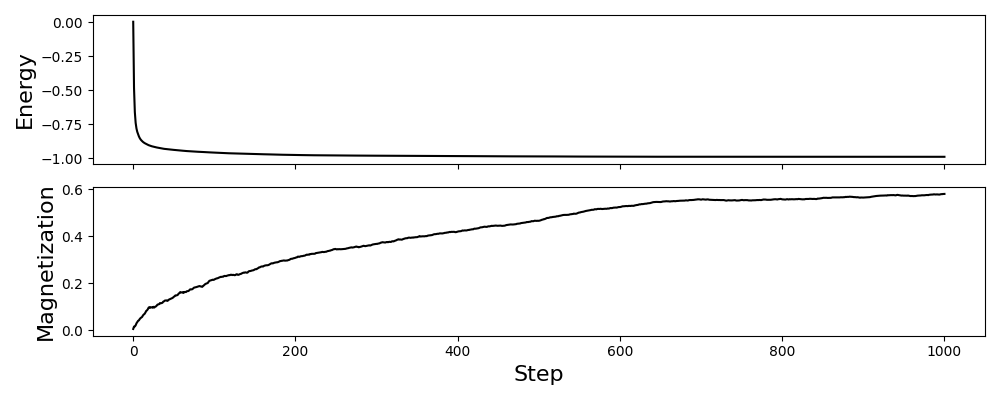
\includegraphics[width=\textwidth]{report_mcmc_gaussian_measurables}
        \centering
        \caption{\textit{Measurables of samples during the sampling process}}
        \label{fig:mcmc_gaussian_b}
    \end{subfigure}
    \centering
    \caption{\textit{
        MCMC quenching of an initial randomly generated $256 \times 256$ spin 
        lattice sample with $J = 0.5$, $\beta = 10$, and a centered Gaussian 
        magnetic field
        $B_{ij} = 0.01 \exp [-\frac{1}{1024}((i-128)^2 + (j-128)^2)]$. 
    }}
    \label{fig:mcmc_gaussian}
\end{figure}

In the MCMC quenching simulation conducted in \ref{fig:mcmc_gaussian}, we 
observe several expected phenomena. 
The pairwise interactions are clearly exhibited by the clusters of aligned spins 
which form and coalesce as the number of steps grows. 
The prescence of the magnetic field also seems to magnetize the entire lattice, 
as indicated both by the convergence on full spin alignment in 
\ref{fig:mcmc_gaussian_a}, and the increasing magnetization measured in 
\ref{fig:mcmc_gaussian_b}. 

Note that computing the measurables for \ref{fig:mcmc_gaussian_a} and 
\ref{fig:mcmc_gaussian_b} is easy given the explicit spin lattice states 
provided by the sampling process. 
The magnetization is simply the average spin. 
The energy is computed using \ref{isingE}. 
We will see that these measurables are not so easily obtained when using belief 
propagation. 

Plots describing additional simulations are shown in the Supporting Materials. 





\subsection{Belief Propagation}





Message-passing belief propagation algorithms are another way to estimate true 
marginals for general graphical models. 
They are derived from the theory of variable elimination, but are applicable to 
general graphs which may include cycles. 

It turns out that belief propagation is especially effective and simple to 
implement on Ising models. 
This follows from the Boltzmann distribution that defines the joint distribution 
of the Ising model:
\begin{equation}\label{isingJoint}
    \tilde{P}(\vec{\sigma}) = \exp \Bigr [\beta J\sum_i \sum_{j \in adj(i)} \sigma_i \sigma_j + \beta \sum_i \sigma_i B_i \Bigr ]
\end{equation}
It factorizes nicely over the Ising lattice:
\begin{equation}\label{gibbsFactorization}
    \tilde{P}(\vec{\sigma}) = \prod_i \exp \Bigr [\beta \sigma_i B_i \Bigr ] \prod_{j \in adj(i)} \exp \Bigr [ \beta J \sigma_i \sigma_j \Bigr ]
\end{equation}
This defines a factor graph of node and edge potentials representing the unary 
and pairwise potentials, respectively:
\[
    \phi_i = \exp \Bigr [\beta \sigma_i B_i \Bigr ]
    \qquad \qquad
    \phi_{ij} = \exp \Bigr [ \beta J \sigma_i \sigma_j \Bigr ]
\]
We then run a standard belief propagation routine. 

\begin{figure}
    \begin{subfigure}{\textwidth}
        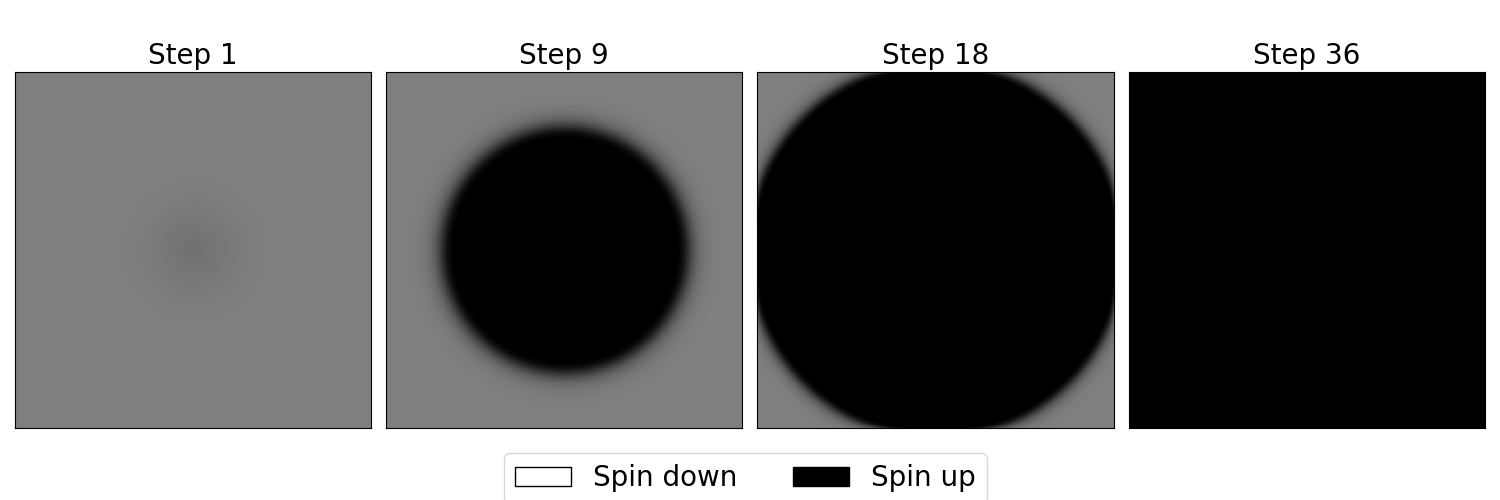
\includegraphics[width=\textwidth]{report_bp_gaussian}
        \centering
        \caption{\textit{Spin lattice beliefs from various steps in the belief propagation process}}
        \label{fig:bp_gaussian_a}
    \end{subfigure}
    \begin{subfigure}{\textwidth}
        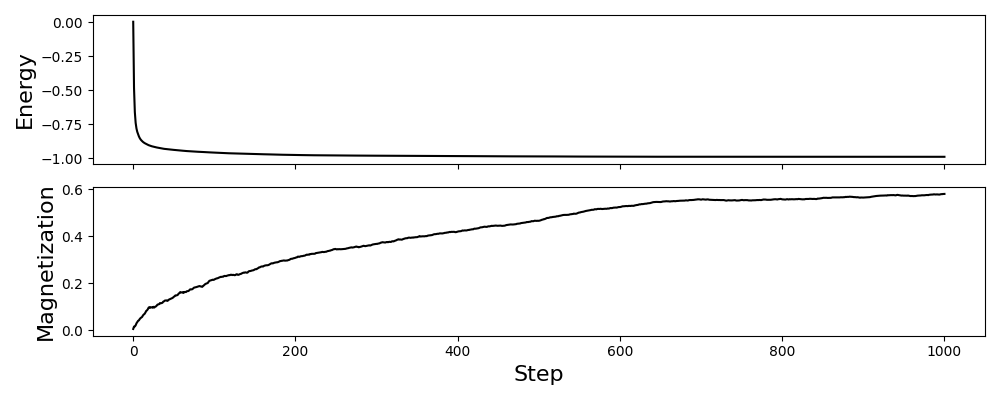
\includegraphics[width=\textwidth]{report_mcmc_gaussian_measurables}
        \centering
        \caption{\textit{Measurables of samples during the sampling process}}
        \label{fig:bp_gaussian_b}
    \end{subfigure}
    \centering
    \caption{\textit{
        Belief propagation to estimate marginal distributions of spin lattice 
        with $J = 0.5$, $\beta = 10$, and a centered Gaussian 
        magnetic field
        $B_{ij} = 0.01 \exp [-\frac{1}{1024}((i-128)^2 + (j-128)^2)]$. 
    }}
    \label{fig:bp_gaussian}
\end{figure}

\newpage

%%%%%%%%%%%%%%%%%%%%%%%%%%%%%%%%%%%%%%%%%%%%%%%%%%%%%%%%%%%%

\end{document}